\subsection{数据访问对象模式}

数据访问对象模式用于把低级的数据访问API或操作从高级的业务服务中分离出来。在本项目中,使用数据访问对象模式将单条的traceLog信息进行包装形成TraceLogMO类。设计TraceLogDao接口并配备TraceLogDaoImpl类实现该接口,该类作为数据访问实体类来进行数据访问工作,并在之后供数据传输模块调用。

\begin{figure}[htb]
  \centering
  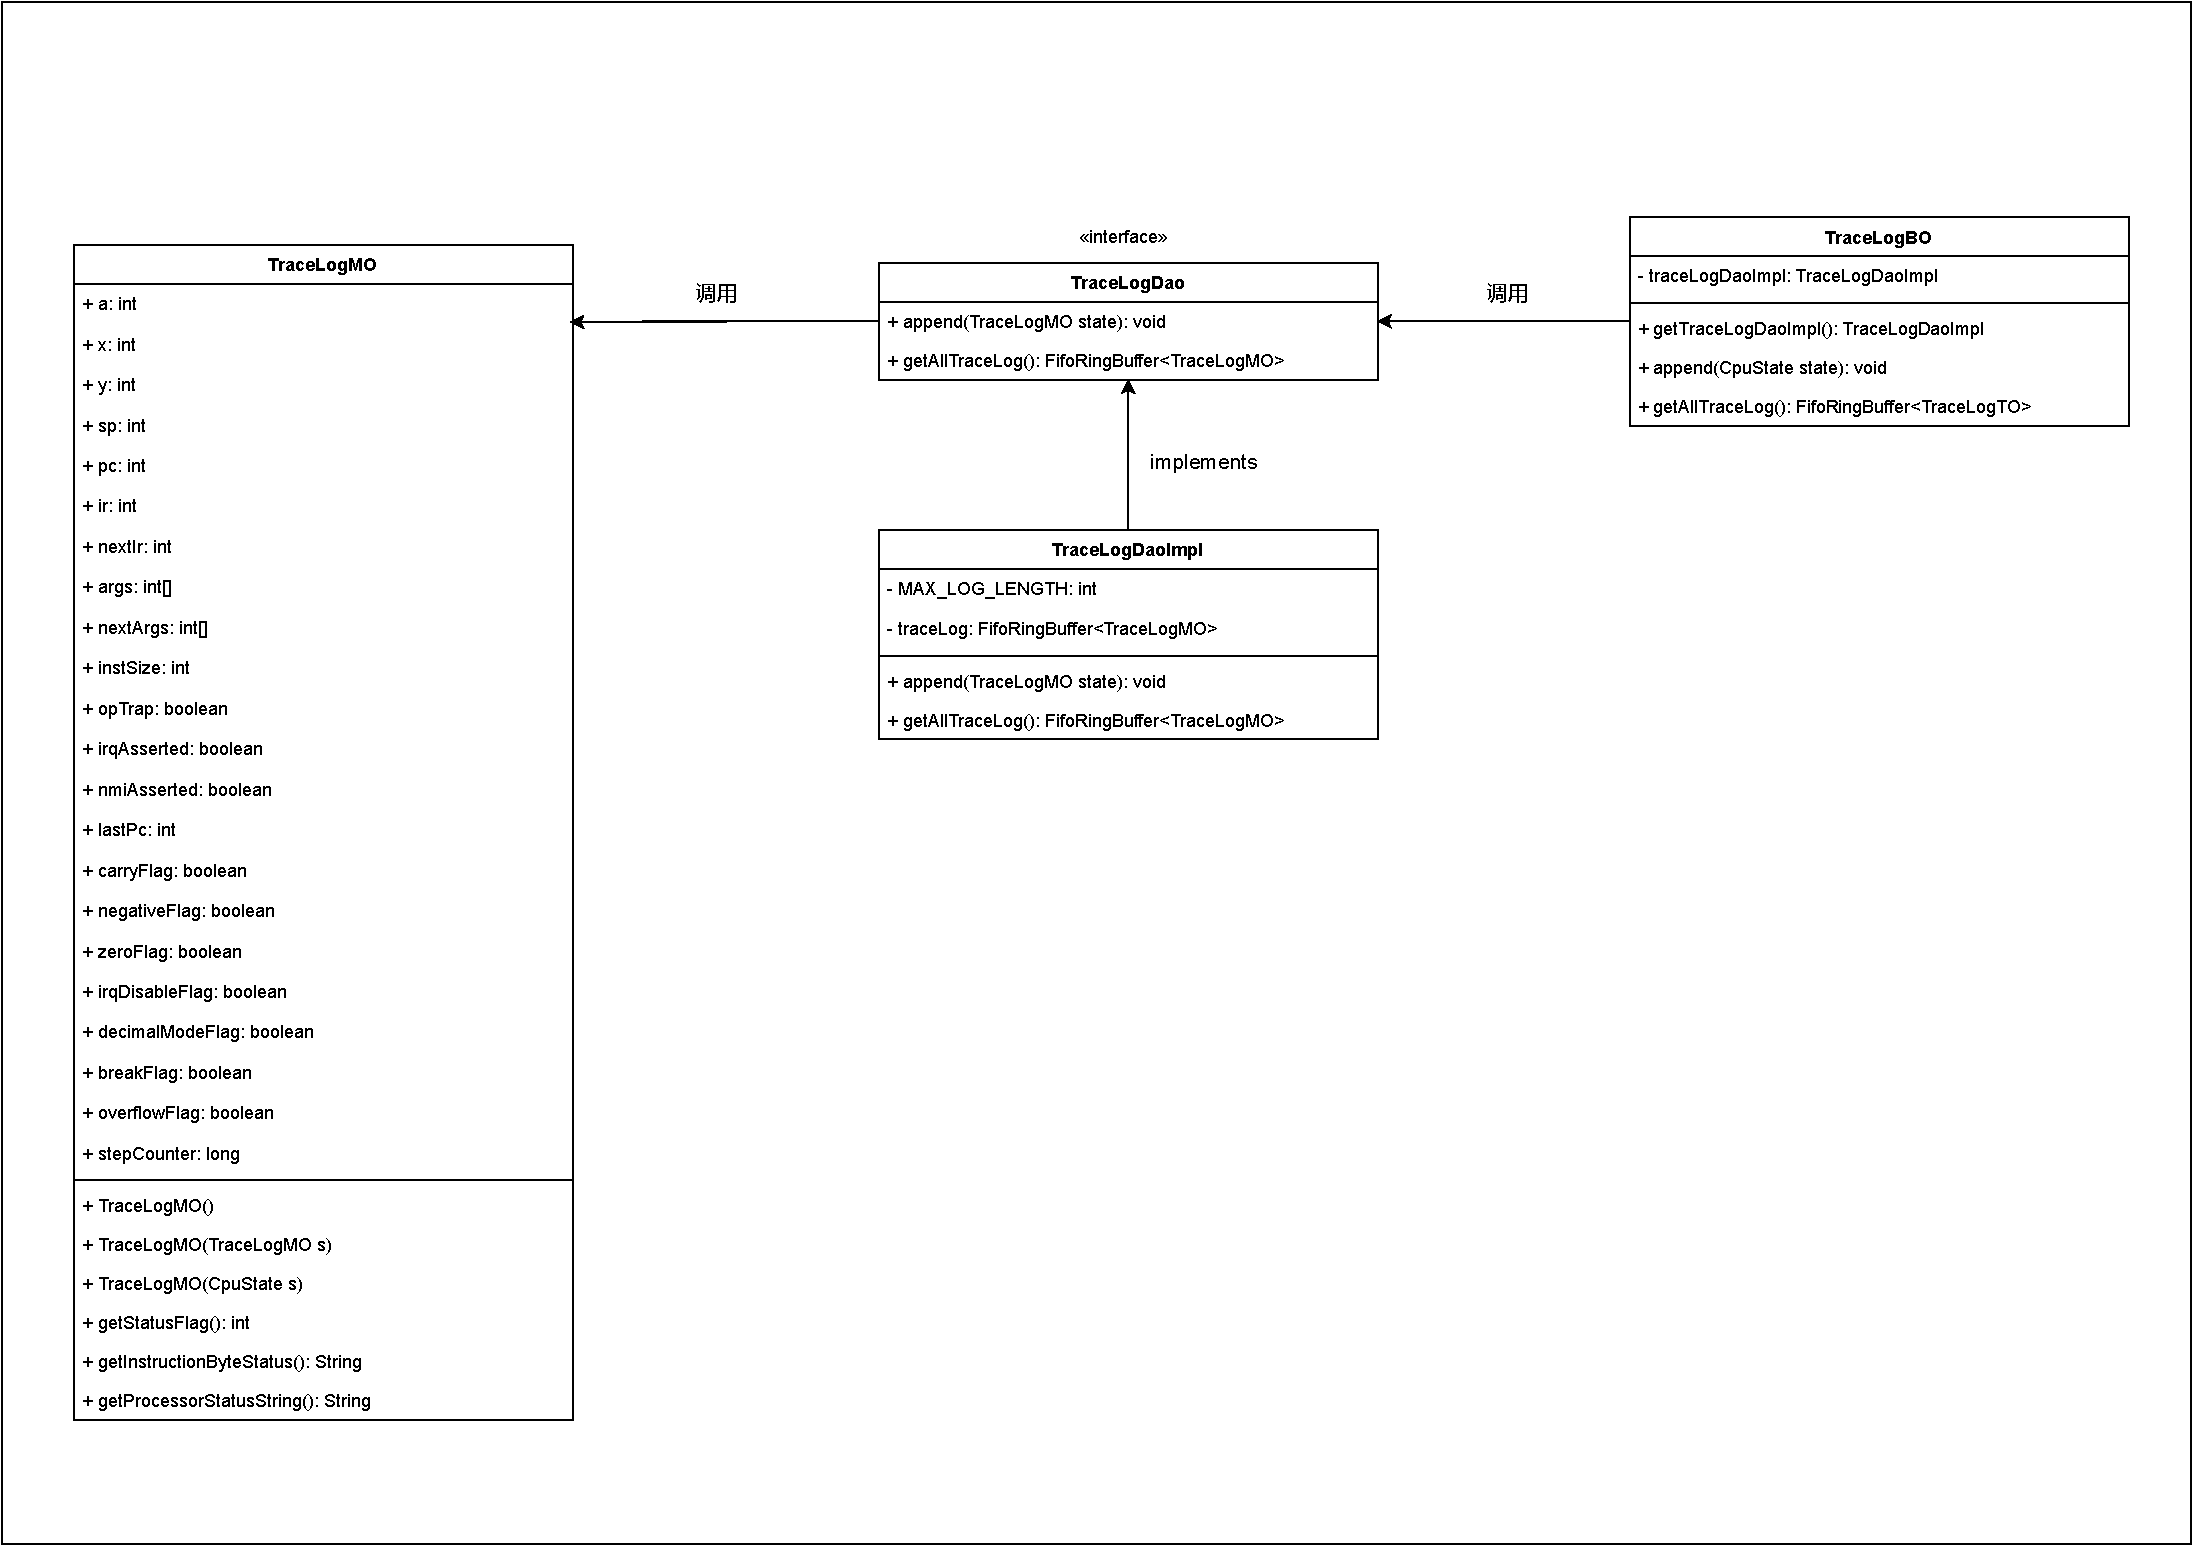
\includegraphics[width=0.9\textwidth]{figures/数据访问对象模式.pdf}
  \caption{数据访问对象模式在 Slow6502 中的类图}
\end{figure}
